\chapter{Evaluation and Alternative Methods}

\section{Evaluation}
\label{sec:evaluation}

As the dataset was already pre-split into training and testing data, we just used the test data to evaluate the best model from our hyperparameter tuning.
The results of the model evaluation are shown in \autoref{tab:evaluation}.

\begin{table}[H]
    \centering
    \resizebox{0.5\textwidth}{!}{%
    \begin{tabular}{|c|c|c|c|c|c|}
        \hline
         Loss & Accuracy & Precision & Recall & F1-Score \\ \hline
         0.01504 & 0.99656 & 0.99939 & 0.99545 & 0.99741 \\ \hline
    \end{tabular}}
    \caption{Evaluation results for model built on top of the frozen \texttt{VGG16} base.}
    \label{tab:evaluation}
    \end{table}


It is immediately apparent that the accuracy is incredibly high.
This is always a bit suspicious, so we are going to look at the probability histogram and confusion matrix, shown in \autoref{fig:eval2}, to see if there are any issues.

\begin{figure}[H]
    \centering
    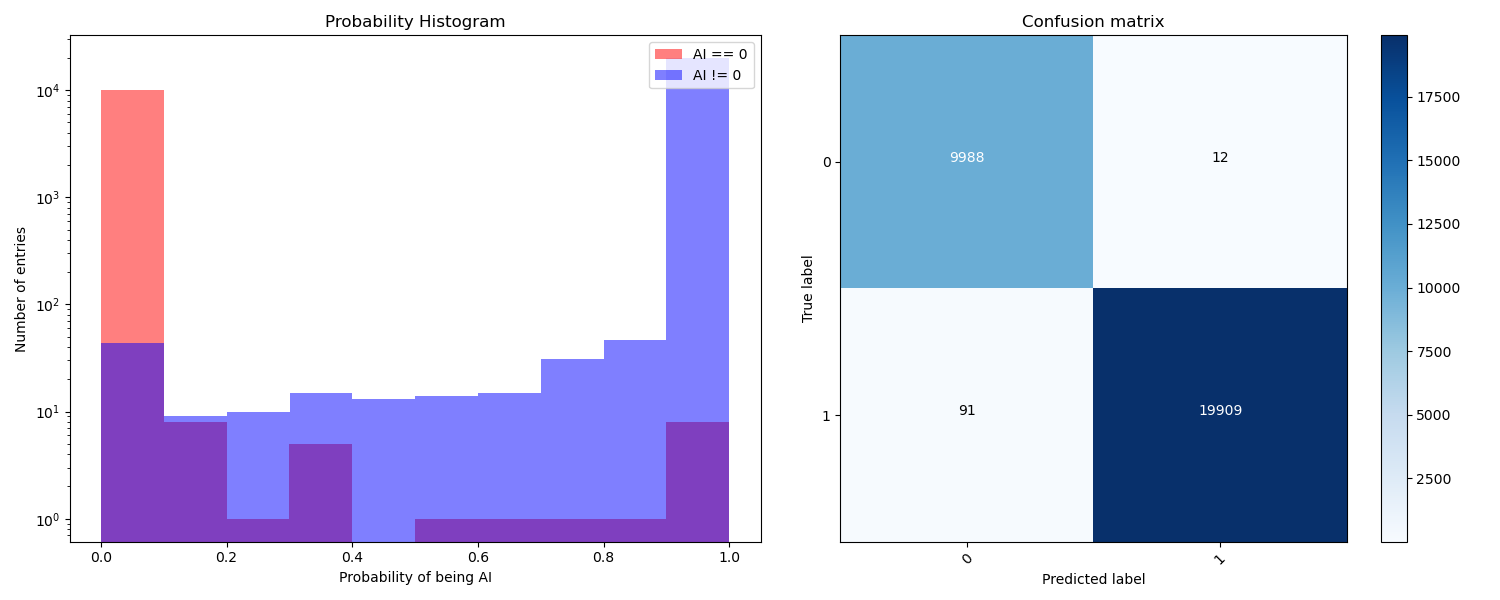
\includegraphics[width=1\textwidth]{images/confusion_matrix_and_histogram.png}
    \caption{The confusion matrix and probability histogram of the our best model.}
    \label{fig:eval2}
\end{figure}

We can see that there are almost no false classifications, with only $91$ AI generated images being classified as human drawn and $12$ vice versa.
As there are so few false classifications, it is all the more intriguing to see which images did still end up being classified incorrectly, 
here shown in \autoref{fig:false_class_AI} and \autoref{fig:false_class_human}.

\begin{figure}[h!]
    \centering
    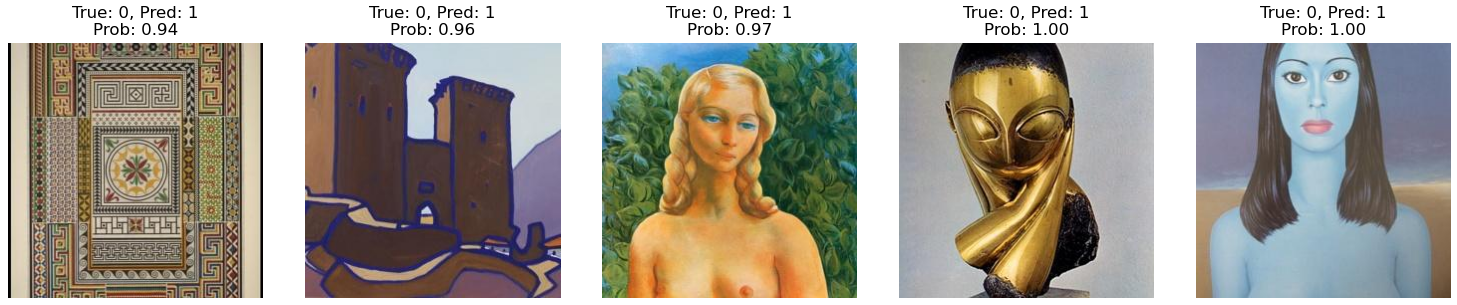
\includegraphics[width=.8\textwidth]{images/top_misclassified_img.png}
    \caption{Examples of human drawn images falsely classified as AI generated \cite{aiartbench}.}
    \label{fig:false_class_AI}
\end{figure}

\begin{figure}[h!]
    \centering
    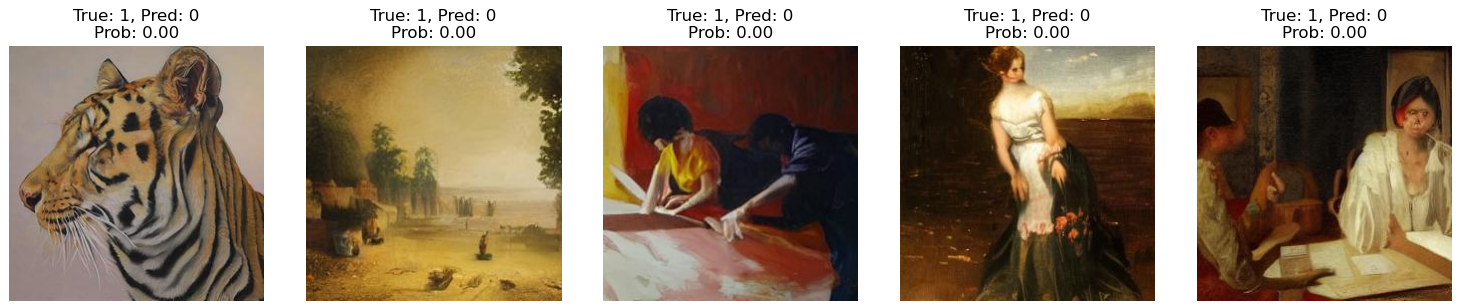
\includegraphics[width=.8\textwidth]{images/bot_misclassified_img.png}
    \caption{Examples of AI generated images falsely classified as human drawn \cite{aiartbench}.}
    \label{fig:false_class_human}
\end{figure}

The following is just a personal impression, but it seems quite understandable the falsely classified images were misclassified, 
although the difference is still quite clear upon closer inspection.
Especially the second image in \autoref{fig:false_class_human} does not immediately strike one as AI generated. \\

What \autoref{fig:eval2} also shows is something that somehow slipped our mind at some point between the preprocessing and the creation of our models:
the test data and the dataset in general is quite unbalanced, with twice as many AI generated images.
This is not a great problem if the model is trained on the entire dataset as there is a lot of images, but it becomes much more apparent
if we more closely inspect how the model behave with singular epochs of art, thus far fewer images.
If we inspect the loss and accuracy curves for those candidates, we can observe a prime example of overfitting.
An example of this can be seen in \autoref{fig:overfitting}.

\begin{figure}[h!]
    \centering
    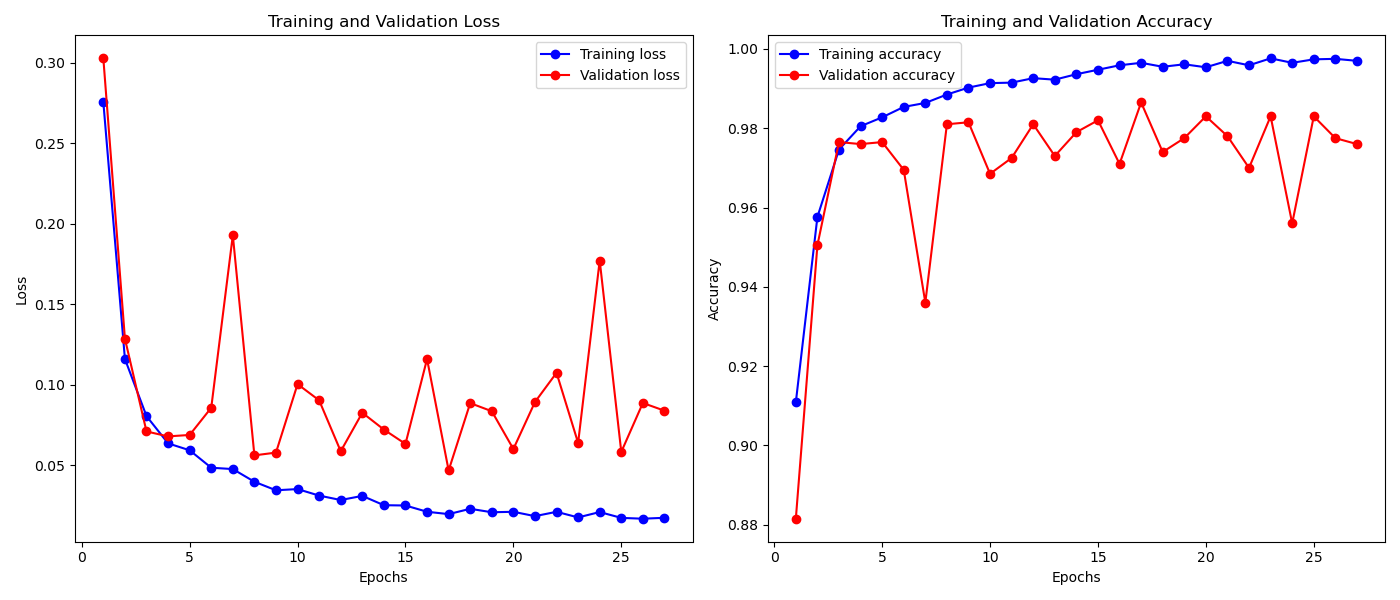
\includegraphics[width=1\textwidth]{images/example_overfitting_baroque.png}
    \caption{Loss and accuracy curves for the model trained on the Baroque epoch. While the training accuracy continues to increase with ongoing epochs, the validation accuracy stagnates.}
    \label{fig:overfitting}
\end{figure}

Similar behaviour can be observed for the other epochs as well, but the Baroque epoch shows this the best. \\

Taking this a step further, we also decided to test the behaviour of models trained on a single epoch but evaluated on the entire dataset, as shown in \autoref{fig:epochs}.

\begin{figure}[h!]
    \centering
    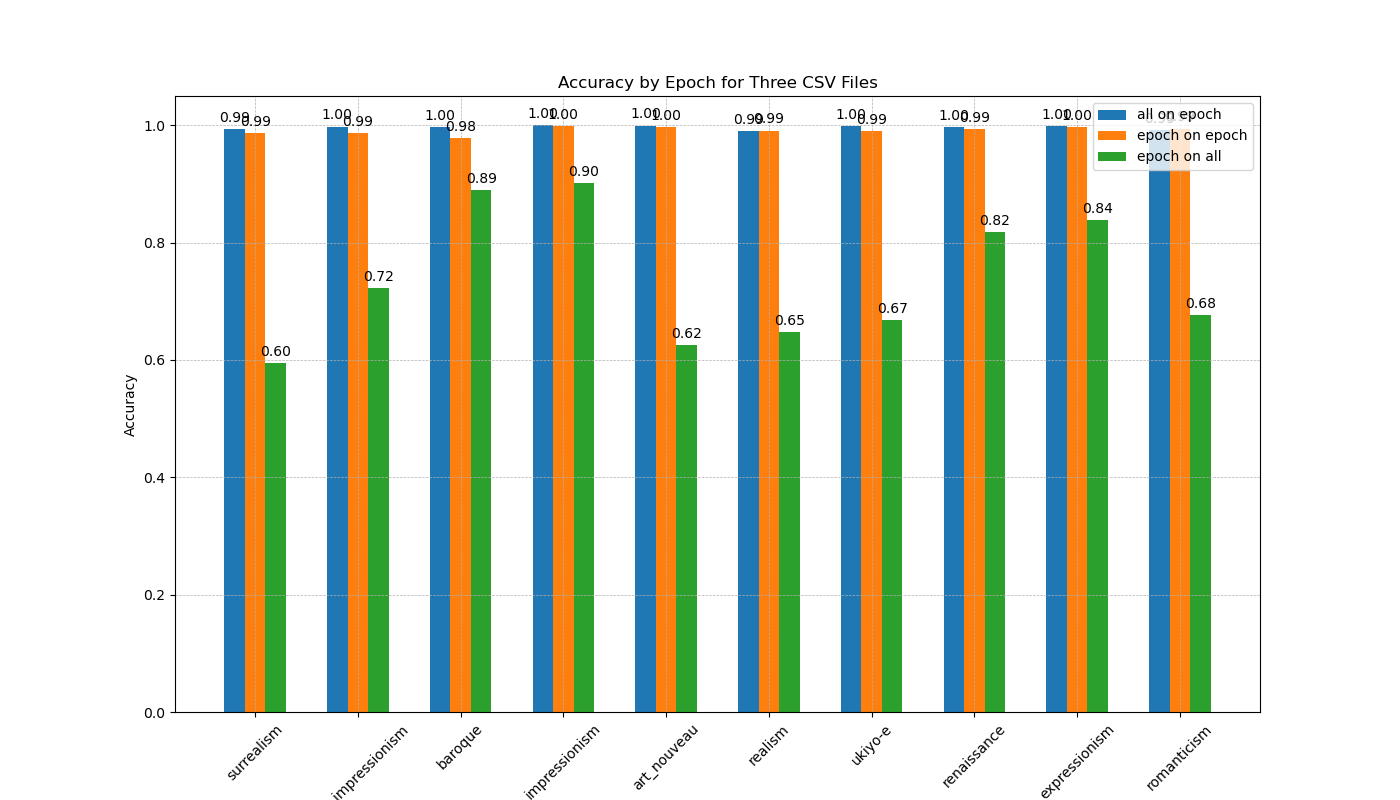
\includegraphics[width=1\textwidth]{images/accuracy_by_epoch.png}
    \caption{Accuracy of the model on art from different epochs trained in three different ways. The blue bars represent the accuracy of the model trained on the entire dataset,
     the orange bars represent the accuracy of the model if trained and evaluated on a single epoch 
     and the green bars represent the accuracy of the models trained on a single epoch but evaluated on the entire dataset.}
    \label{fig:epochs}
\end{figure}

This shows that the global model performs almost perfectly on all and the models trained on a single epoch perform great on their own epoch, as is to be expected,
but the models trained on a single epoch and evaluated on the entire dataset performed sometimes only slightly better than random guessing.
A cause of this could in theory be greatly differing art styles between the epochs, but it is much more likely that the models
are simply overfitted to the training data. \\

\section{Comparison to Alternative Methods}

In addition to the previously discussed method, we also decided to compare our model to a few alternative methods.
First, we took an image classifier from GitHub created by user \textit{Piyush Yadav} \cite{github_model}.
This classifier, similarly to our model, utilised a CNN to classify the images.
Differently however, this model was trained on generated and real photographs instead of AI generated and human drawn art.
It did not seem promising to just apply the model to our dataset, but we were still interested in how it would perform.
After applying the model to our dataset, we achieved an accuracy of barely $31 \%$, which is quite a bit worse than even random guessing.
As already noted, this is not all that surprising, considering the model was trained to solve a (if only minisculely) different task.
Also, the alternative model was trained on a dataset of much lower resolution, so, while for our model the resolution did not quite matter, it cannot be ruled out
that this was also a cause of the low accuracy in addition to the possibility that the features setting real and fake images apart are just really different between
art and photographs.   \\

The second alternative we tried was the already mentioned model by Kaggle user \textit{nibrastuhh} \cite{useraiartbench}, who published the dataset we used.
Compared to our model, this model was much simpler, consisting of only a few layers, especially after taking the extra layers from \texttt{VGG16} into account,
yet still achieved an accuracy of over $90 \%$.
Their model also did not run into the same stability issues as ours, which is likely helped by them actually balancing the dataset beforehand.
Still, our model achieved an even higher accuracy, so we can be content with our results. \\

Lastly, we tried a random forest classifier, which is a much simpler model than a CNN.
After some testing, this classifier achieved an accuracy of around $75 \%$, which is not bad considering its simplicity, but by far not as good of a result as our model.
This shows what could already be anticipated from the start: CNNs are much better suited for this type of image classification than classical methods,
especially when it comes to large amounts of data. \\

\section{Conclusion and Outlook}

In conclusion, we managed to, after a lot of trial and error, create a model that did not show the initial instability issues encountered before and achieved a very high accuracy.
This model achieved an accuracy of over $99 \%$ on the test data, all while performing just as well on the individual epochs of art,
even when compared to models trained on a single epoch.

Despite the results we achieved, there is still a lot of room for future improvement.
Firstly, it would be nice to balance the dataset, optimally not by throwing away the imbalance, but instead by collecting more hand drawn images.
This would likely also help with the overfitting issue we encountered.
It would also be interesting to try out the approaches that were discarded for time and resource problems, such as using cross-validation and/or a lower learning rate.
Furthermore, a model that is both able to differentiate generated and real images as well as photographs would be interesting.
It also remains to be seen how well the model holds up against new AI generated images, as their quality is improving at a high pace.


